\section{Discussion}
% ──────────────────────────────────────────────────────────────────────────────

The results reveal both encouraging convergences and persistent gaps in how
medical XAI is currently evaluated. This section interprets the key findings,
proposes a minimal evaluation framework, discusses threats to validity, and
identifies directions for future research.

% ──────────────────────────────────────
\subsection{Interpretation of Key Findings}

Expanding the corpus to 52 studies introduces an important revision to the
Faithfulness finding. Rather than appearing universally, Faithfulness was
present in 47 of 52 studies (90.4\%), with the five exceptions
concentrated in human-centred and consistency-focused
designs~\cite{rezaeian2026explainability,finzel2024human,bauer2025human,qin2025consistency,alpsalaz2026explainability}.
This pattern is analytically significant: Faithfulness absence is not
randomly distributed but co-occurs with a shift in evaluation layer,
indicating a genuine conceptual divide between technical-fidelity and
clinician-trust research paradigms. Studies prioritising clinician-facing
evaluation appear to operate under a distinct evaluative logic in which
mathematical fidelity to the model is not the primary concern---a finding
consistent with Rosenfeld's~\cite{rosenfeld2021better} observation that
technical and human-centred evaluation priorities tend to diverge.

Because Faithfulness now exhibits non-trivial variance across the corpus,
Spearman correlations involving it are computable. The
Faithfulness--Sensitivity correlation is modest but statistically significant
($\rho = 0.33$, $p = 0.016$), confirming co-occurrence without implying full
redundancy. The strongest pairwise relationship in the corpus is between
AOPC/MoRF and Pixel Flipping ($\rho = 0.51$, $p < 0.001$), a result that is
mechanistically expected: both are pixel-level perturbation methods that
degrade saliency-ranked features and measure the resulting prediction drop.
AOPC/MoRF and IROF also correlate significantly ($\rho = 0.37$, $p = 0.007$).
These correlations suggest that reporting all three perturbation metrics may
add limited incremental information while increasing methodological
complexity. However, this interpretation should be qualified: co-occurrence
correlation does not establish construct equivalence, and further empirical
work is needed to determine whether these metrics yield convergent results
on the same datasets and explanation methods.

\begin{figure}[H]
  \centering
  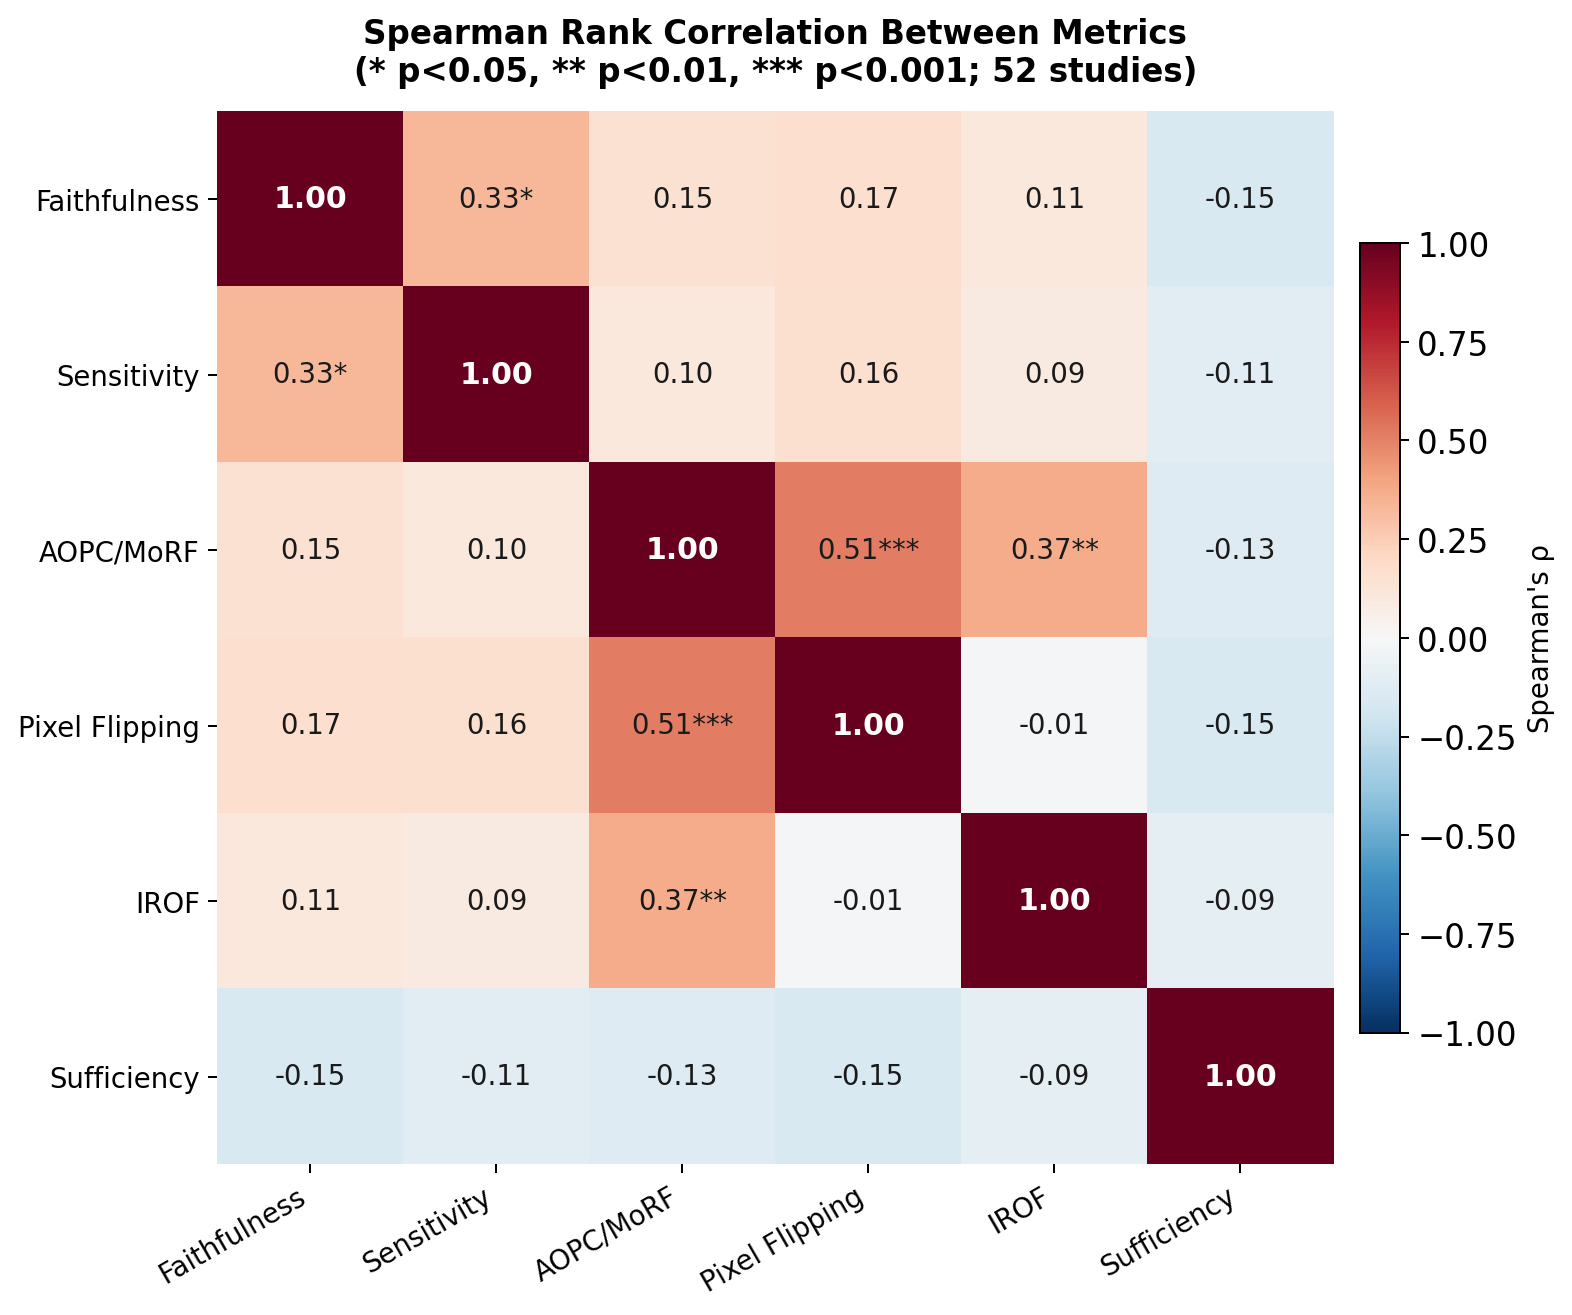
\includegraphics[width=0.85\linewidth]{fig4_spearman_correlation}
  \caption{Spearman rank correlation ($\rho$) between XAI evaluation metrics
  across the 52-study corpus. In the binary encoding used here, Spearman's
  $\rho$ is mathematically equivalent to the phi coefficient ($\phi$).
  Statistical significance is indicated as: ${}^{*}p < 0.05$,
  ${}^{**}p < 0.01$, ${}^{***}p < 0.001$. The AOPC/MoRF--Pixel Flipping
  pair exhibits the strongest correlation ($\rho = 0.51$), while Sufficiency
  shows negative (non-significant) correlations with all other metrics.}
  \label{fig:spearman_correlation}
\end{figure}

The isolation of Sufficiency remains noteworthy. It appeared in only 4 of 52
studies (7.7\%)---a proportion essentially unchanged from smaller prior
corpora---and exhibited negative correlations with all other metrics
($\rho$ ranging from $-0.09$ to $-0.15$, all non-significant). Its low
co-occurrence likely reflects a conceptual gap rather than merely an adoption
lag. Sufficiency asks whether the features identified as important are, on
their own, sufficient to reproduce the model's prediction (see
Equation~\ref{eq:sufficiency})---a question of direct clinical relevance
that the remaining metrics do not address. This disconnect echoes the broader
critique by Kadir et al.~\cite{kadir2023evaluation} that human-centred and
decision-adequacy assessment remains underdeveloped relative to technical
faithfulness metrics.

The sub-domain disparity between oncology and neuroimaging further
underscores that metric richness is unevenly distributed. Oncology
benefits from well-established imaging benchmarks that support diverse
evaluation protocols, whereas neuroimaging lacks analogous shared resources,
which likely constrains both metric diversity and cross-study comparability.
This disparity suggests that targeted benchmark development for underserved
sub-domains could have a disproportionately positive effect on evaluation
standardisation.

% ──────────────────────────────────────
% [ADDED SECTION — Minimal Evaluation Framework]
\subsection{Toward a Minimal Evaluation Framework}

Building on the co-occurrence patterns, correlation analysis, and taxonomy
mapping reported above, we propose a minimal evaluation framework for medical
XAI that spans all three taxonomy layers while imposing a tractable
methodological burden. The framework specifies five evaluation dimensions,
each addressed by at least one metric:

\begin{enumerate}
    \item \textbf{Faithfulness} (Layer~1). One faithfulness metric (e.g.,
    Faithfulness Correlation as defined in Equation~\ref{eq:faithfulness})
    should be reported to establish that the explanation reflects the model's
    actual decision-making process. Faithfulness is the most widely adopted
    metric (90.4\% of corpus) and serves as the foundation for technical
    credibility.

    \item \textbf{Perturbation-based fidelity} (Layer~1). One
    perturbation-based metric---AOPC (Equation~\ref{eq:aopc}), Pixel Flipping
    (Equation~\ref{eq:pixel_flipping}), or IROF
    (Equation~\ref{eq:irof})---should be reported to validate that the
    explanation identifies features whose removal degrades model performance.
    Given the observed redundancy among perturbation metrics ($\rho = 0.51$
    for AOPC--Pixel Flipping), reporting a single perturbation metric is
    typically sufficient. IROF is recommended when explanations operate on
    semantically coherent regions rather than individual pixels.

    \item \textbf{Sensitivity} (Layer~1/2). One sensitivity metric (e.g.,
    Max-Sensitivity, Equation~\ref{eq:sensitivity}) should be reported to
    assess explanation stability under input perturbation. Sensitivity bridges
    Layer~1 and Layer~2, as it captures both the mathematical responsiveness
    of the explanation and its robustness to noise.

    \item \textbf{Sufficiency} (Layer~1). One sufficiency metric
    (Equation~\ref{eq:sufficiency}) should be reported to determine whether
    the explanation identifies a feature subset that alone sustains the
    model's prediction. Sufficiency is currently the most underutilised metric
    in the corpus (7.7\%) yet directly addresses the clinically important
    question of whether the explanation captures decision-adequate evidence.

    \item \textbf{Human-centred evaluation} (Layer~3). At least one
    human-centred measure---such as clinician trust calibration, cognitive
    load assessment, or diagnostic decision accuracy---should be reported
    to validate that the explanation provides practical value in clinical
    workflows. Only 13.5\% of corpus studies currently address this dimension.
\end{enumerate}

This five-component framework is designed to be both comprehensive and
parsimonious. It ensures coverage of all three taxonomy layers without
requiring the simultaneous application of all six identified metrics, several
of which exhibit partial redundancy. Researchers operating under resource
constraints may prioritise components 1, 2, and 5 as a minimum viable set,
provided that the omission of sensitivity and sufficiency is explicitly
acknowledged and justified.

% ──────────────────────────────────────
% [ADDED SECTION — Threats to Validity]
\subsection{Threats to Validity}

Several threats to the validity of this study should be considered.

\paragraph{Internal Validity.}
The classification of evaluation metrics into canonical categories requires
interpretive judgement. Although we followed established normalisation
procedures grounded in prior
literature~\cite{rosenfeld2021better,kadir2023evaluation}, different coding
decisions could alter the metric distribution. The binary encoding of metric
presence (1/0) discards information about the depth or quality of metric
application within each study: a study that reports Faithfulness as its
central evaluation axis is coded identically to one that mentions it
peripherally. Additionally, the screening process, while conducted by two
independent reviewers with substantial agreement (Cohen's $\kappa = 0.82$),
is not immune to selection bias; studies published in languages other than
English, or in venues not indexed by the searched databases, may have been
missed.

\paragraph{External Validity.}
The corpus of 52 studies spans five medical sub-domains but remains modest
in absolute size. The observed patterns should therefore be interpreted as
indicative of current trends rather than definitive characterisations, and
require replication on larger systematically assembled samples. The
restriction to medical XAI, while analytically necessary to ensure
domain-specific relevance, limits the generalisability of the findings to
other high-stakes domains such as autonomous driving or financial risk
assessment. Evidence from non-medical
applications~\cite{Ghosh2024DemystifyingEC,Nagy2024ImprovingUM} suggests
that similar metric fragmentation may exist in other domains, but this
remains to be systematically investigated.

\paragraph{Construct Validity.}
The co-occurrence analysis captures which metrics tend to appear together
but cannot establish whether two frequently co-occurring metrics are
genuinely redundant (i.e., measuring the same underlying construct) or
merely reported together by convention. The Spearman correlations reported
here measure association in usage patterns, not agreement in evaluation
outcomes. Establishing true redundancy would require applying multiple
metrics to the same explanation--dataset pairs and comparing their
outputs---a task outside the scope of the present review. Furthermore, the
taxonomy's three layers were constructed primarily through deductive reasoning
from prior literature. While the corpus mapping provides partial empirical
validation, a prospective study with clinical practitioners would be needed
to confirm that the human-centred trust layer adequately captures what domain
experts actually require from explanations.

% ──────────────────────────────────────
\subsection{Limitations}

Several additional limitations qualify these findings. First, the corpus
size of 52 studies, while sufficient for identifying broad distributional
patterns, limits the statistical power of pairwise correlation analyses,
particularly for low-frequency metrics such as IROF and Sufficiency (each
$n = 4$). Correlations involving these metrics should be interpreted with
caution. Second, the study does not include direct clinician validation of
the proposed taxonomy or minimal evaluation framework; while both are
grounded in empirical usage patterns and prior theoretical frameworks,
prospective user studies are needed to confirm their practical utility in
clinical evaluation workflows. Third, the degree of metric redundancy
inferred from co-occurrence patterns remains uncertain without
head-to-head comparisons on shared datasets; co-occurrence in reporting
practices is a necessary but not sufficient condition for construct overlap.
Fourth, our corpus prioritises English-language publications in indexed
venues, which may underrepresent evaluation practices in non-English-speaking
research communities.

% ──────────────────────────────────────
\subsection{Future Work}

Three directions follow from the present findings. First, a prospective
study instrumenting clinicians as they interact with SHAP- and
Grad-CAM-generated explanations would ground the trust layer of the taxonomy
in behavioural evidence and provide the clinician validation that the
current study lacks. Second, developing a standardised reporting template
for medical XAI evaluations---specifying the minimal metric set proposed in
Section~6.2 alongside optional domain-specific additions---could reduce the
fragmentation documented in this review and improve cross-study
comparability. Third, extending future analyses to include user-study metrics
such as cognitive load and decision accuracy would enable empirical testing
of whether high Faithfulness scores translate into genuine clinical
utility---a question the current literature leaves largely unanswered.


\section{Conclusion}
% ──────────────────────────────────────────────────────────────────────────────

This paper investigated the evaluation landscape of XAI within the medical
domain, focusing on how quantitative metrics co-occur and distribute across
oncology, cardiology, neuroimaging, radiology, and clinical decision support.
Drawing on a systematically assembled corpus of 52 peer-reviewed studies, we
identified a dominant cluster of technically grounded
metrics---Faithfulness and Sensitivity---that consistently co-occur and
collectively account for the majority of evaluation activity.
Perturbation-based metrics such as AOPC/MoRF and Pixel Flipping form a
correlated secondary cluster ($\rho = 0.51$, $p < 0.001$), while
Sufficiency remains an isolated and underutilised criterion (7.7\%) despite
its direct relevance to clinical decision adequacy.

Mapping the corpus onto a three-layer taxonomy of mathematical faithfulness,
system robustness, and human-centred trust confirmed that current evaluation
practice is heavily concentrated in the first layer: 90.4\% of studies
addressed mathematical faithfulness, but only 34.6\% addressed system
robustness and 13.5\% included any human-centred criterion,
leaving substantial gaps in the dimensions most consequential
for clinical deployment.

These findings support two main conclusions. First, a minimal but
comprehensive evaluation framework---combining one faithfulness measure, one
perturbation-based measure, one sensitivity metric, one sufficiency check,
and at least one human-centred criterion---would cover all three taxonomy
layers without imposing an unreasonable methodological burden. Second, the
field requires shared benchmarks and reporting standards that make
cross-study comparison tractable, particularly for underserved sub-domains
such as neuroimaging, where evaluation practice currently lags behind more
established areas. Addressing these gaps is a necessary step toward medical
AI systems whose explanations are not only technically faithful but genuinely
trustworthy in clinical practice.

\newpage
% ─────────────────────────────────────────────────────────────────────────────
